%%%%%%%%%%%%%%%%%%%%%%%%%%%%%%%%%%%%%%%%%
% * <rodrigosanchez@ciencias.unam.mx> 2018-06-04T08:35:40.012Z:
%
% ^.
% Beamer Presentation
% LaTeX Template
% Version 1.0 (10/11/12)
%
% This template has been downloaded from:
% http://www.LaTeXTemplates.com
%
% License:
% CC BY-NC-SA 3.0 (http://creativecommons.org/licenses/by-nc-sa/3.0/)
%
%%%%%%%%%%%%%%%%%%%%%%%%%%%%%%%%%%%%%%%%%

%----------------------------------------------------------------------------------------
%	PACKAGES AND THEMES
%----------------------------------------------------------------------------------------

\documentclass{beamer}

\mode<presentation> {

% The Beamer class comes with a number of default slide themes
% which change the colors and layouts of slides. Below this is a list
% of all the themes, uncomment each in turn to see what they look like.

%\usetheme{default}
%\usetheme{AnnArbor}
%\usetheme{Antibes}
%\usetheme{Bergen}
%\usetheme{Berkeley}
%\usetheme{Berlin}
%\usetheme{Boadilla}
%\usetheme{CambridgeUS}
%\usetheme{Copenhagen}
%\usetheme{Darmstadt}
%\usetheme{Dresden}
%\usetheme{Frankfurt}
%\usetheme{Goettingen}
%\usetheme{Hannover}
\usetheme{Ilmenau}
%\usetheme{JuanLesPins}
%\usetheme{Luebeck}
%\usetheme{Madrid}
%\usetheme{Malmoe}
%\usetheme{Marburg}
%\usetheme{Montpellier}
%\usetheme{PaloAlto}
%\usetheme{Pittsburgh}
%\usetheme{Rochester}
%\usetheme{Singapore}
%\usetheme{Szeged}
%\usetheme{Warsaw}

% As well as themes, the Beamer class has a number of color themes
% for any slide theme. Uncomment each of these in turn to see how it
% changes the colors of your current slide theme.

%\usecolortheme{albatross}
%\usecolortheme{beaver}
%\usecolortheme{beetle}
%\usecolortheme{crane}
%\usecolortheme{dolphin}
%\usecolortheme{dove}
%\usecolortheme{fly}
%\usecolortheme{lily}
%\usecolortheme{orchid}
%\usecolortheme{rose}
%\usecolortheme{seagull}
%\usecolortheme{seahorse}
%\usecolortheme{whale}
%\usecolortheme{wolverine}

%\setbeamertemplate{footline} % To remove the footer line in all slides uncomment this line
%\setbeamertemplate{footline}[page number] % To replace the footer line in all slides with a simple slide count uncomment this line

%\setbeamertemplate{navigation symbols}{} % To remove the navigation symbols from the bottom of all slides uncomment this line
}

\usepackage[spanish]{babel}
\usepackage[utf8]{inputenc}
\usepackage{wrapfig}
\usepackage{ragged2e}
\apptocmd{\frame}{}{\justifying}{} % Allow optional arguments after frame.
\selectlanguage{spanish}
\usepackage{CJKutf8} % Pa'l japonés.
\usepackage{graphicx} % Allows including images
\usepackage{booktabs} % Allows the use of \toprule, \midrule and \bottomrule in tables
\usepackage{minted} % Para código en Haskell
\setminted{fontsize=\footnotesize, baselinestretch=1}

%----------------------------------------------------------------------------------------
%	TITLE PAGE
%----------------------------------------------------------------------------------------

\title[Ensemble Computation]{Ensemble Computation} % The short title appears at the bottom of every slide, the full title is only on the title page

\author{Rodrigo Alejandro Sánchez Morales} % Your name
\institute[UNAM] % Your institution as it will appear on the bottom of every slide, may be shorthand to save space
{
\makebox[0pt][r]{\raisebox{-\totalheight}[0pt][0pt]{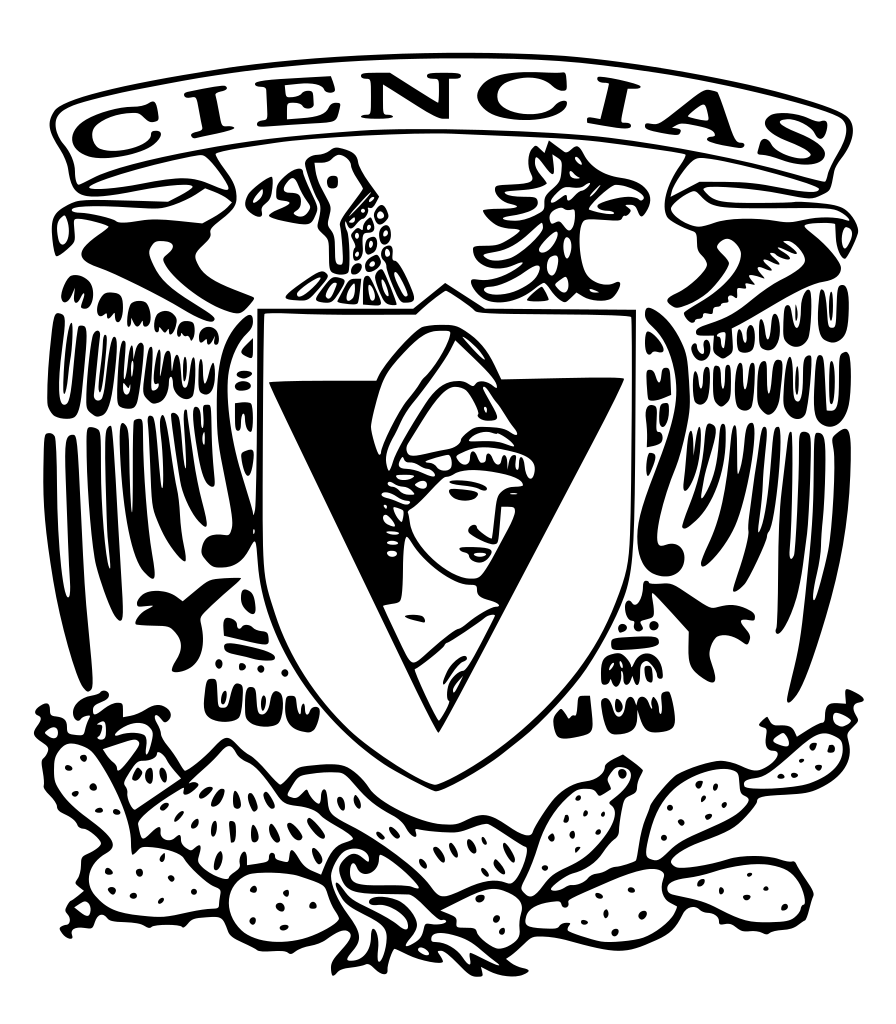
\includegraphics[width=1in]{ciencias}}}
Universidad Nacional Autónoma de México \\ % Your institution for the title page
Facultad de Ciencias \\
\medskip
\textit{Complejidad Computacional, 2019-I} % Your email address
}
\date{Octubre de 2018} % Date, can be changed to a custom date

\begin{document}

\begin{frame}
\titlepage % Print the title page as the first slide
\end{frame}

\begin{frame}
\frametitle{Tabla de contenidos} % Table of contents slide, comment this block out to remove it
\tableofcontents % Throughout your presentation, if you choose to use \section{} and \subsection{} commands, these will automatically be printed on this slide as an overview of your presentation
\end{frame}

%----------------------------------------------------------------------------------------
%	PRESENTATION SLIDES
%----------------------------------------------------------------------------------------

%------------------------------------------------
\section{Introducción} % Sections can be created in order to organize your presentation into discrete blocks, all sections and subsections are automatically printed in the table of contents as an overview of the talk
%------------------------------------------------

\subsection{Reducciones} % A subsection can be created just before a set of slides with a common theme to further break down your presentation into chunks

\begin{frame}
\frametitle{¿Qué es una reducción?}
\begin{block}{Definición:}
Una reducción es una transformación de un problema a otro problema.
\end{block}
\end{frame}

%------------------------------------------------

\begin{frame}
\frametitle{Técnicas para probar la NP-Completez}
    \begin{itemize}
        \item Restriction.
        \item Component Design.
        \item \textbf{Local Replacement:} Todo lo que hacemos es elegir algún aspecto del ejemplar del problema NP-Completo conocido para hacer una colección de unidades básicas, y obtenemos el ejemplar correspondiente al problema objetivo reemplazando cada unidad básica de manera uniforme con una estructura diferente.
    \end{itemize}
\end{frame}

%------------------------------------------------
\section{Vertex Cover}
%------------------------------------------------

\begin{frame}
    \frametitle{¿Qué es el Vertex Cover?}
    Es un conjunto de vértices tales que cada arista del grafo es incidente a al menos un vértice del conjunto.
    \begin{figure}[H]
      \centering
      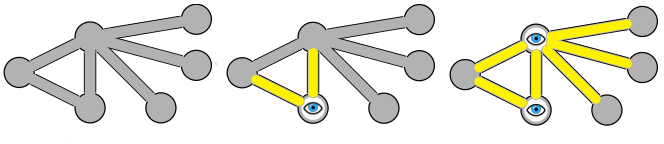
\includegraphics[width=10cm]{coverture}
    \end{figure}
\end{frame}

%------------------------------------------------

\subsection{Descripción del problema}
\begin{frame}{¿Cómo probar NP-Completez?}
\begin{block}{Requisitos}
Para probar que un problema es NP-Completo debemos probar que está en NP, buscar un problema NP-Completo y luego reducirlo a nuestro problema en tiempo polinomial.
\end{block}
%\begin{figure}
%\centering
%  \includegraphics[width=7cm]{reductions}
%\end{figure}
\end{frame}

%------------------------------------------------
\section{Demostración}
%------------------------------------------------

\subsection{}

\begin{frame}
    \frametitle{Representación del problema}
    \begin{block}{Ejemplar:}
        Una colección \textit{C} de subconjuntos de un conjunto finito \textit{A} y un entero positivo \textit{J}.
    \end{block}
    \begin{block}{Pregunta:}
        ¿Hay una secuencia
        \begin{align*}
            <z_1 = x_1 \cup y_1 , z_2 = x_2 \cup y_2, \dots, z_j = x_j \cup y_j>
        \end{align*}
        de $j \leq J$ operaciones de unión, donde cada $x_i$ y $y_i$ es $\{a\}$ para algún $a \in A$ o $z_k$ para algún $k < i$, tal que $x_i$ y $y_i$ son disjuntos a $1 \leq i \leq j$ y que para cad tu subconjunto $c \in C$ hay algún $z_j$, $1 \leq i \leq j$, que es idéntico a $c$? 
    \end{block}
\end{frame}

%------------------------------------------------

\begin{frame}{\textit{Ensemble Computation} es NP-Completo}
    \begin{block}{\textit{Ensemble Computation} \in NP}
            Dado un ejemplar particular del problema, es posible especificar un algoritmo que en la primera fase \textit{adivinadora} asigne un elemento de la secuencia $z_i$ y en la segunda fase \textit{verificadora} compruebe si la asignación resuelve el problema.
    \end{block}
    \begin{flushright}
        $\therefore$ \textit{Ensemble Computation} $\in NP$
    \end{flushright}
\end{frame}

%------------------------------------------------

\begin{frame}
    \begin{block}{Idea principal:}
        Transformamos \textit{Vertex Cover} a \textit{Ensemble Computation}.
    \end{block}
    \begin{center}
        \huge{\textit{Vertex Cover}} \\
        \huge{\propto_p} \\
        \huge{\textit{Ensemble Computation}}
    \end{center}
\end{frame}

%------------------------------------------------

\begin{frame}
    Sea la gráfica $G=(V,E)$ y un entero positivo $K \leq |V|$ que constituye un ejemplar arbitrario de \textit{Vertex Cover}.\\
    
    La unidad básica del ejemplar de \textit{Vertex Cover} son las aristas de $G$. \\
    
    Sea $a_0$ un nuevo elemento no en $V$. \\
    
    El \textbf{reemplazo local} sólo sustituye para cada arista $\{u,v\} \in E$, el subconjunto $\{a_0,u,v\} \in C$.
\end{frame}

%------------------------------------------------

\begin{frame}
    El ejemplar de \textit{Ensemble Computation} está completamente especificado por:
    \begin{align*}
    \huge A &= V \cup {a_0} \\
        C &= \{\{a_0,u,v\}: \{u,v\} \in E\} \\
        J &= K + |E|
    \end{align*}
    Es fácil ver que este ejemplar puede ser construido en tiempo polinomial.
\end{frame}

\begin{frame}
    Afirmamos que $G$ tiene una cubierta de vértices de tamaño $K$ o menos si y sólo si la secuencia deseada de $j \leq J$ operaciones existe para $C$.\\
    \begin{center}
        \huge \textit{G} tiene cubierta de vértices, $|K|$ \\ $\Leftrightarrow$ \\ $\exists$ secuencia $j \leq J$ operaciones $\in C$
    \end{center}
\end{frame}

\begin{frame}
    \underline{$\Rightarrow$} \\
    Primero, supongamos que $V'$ es una cubierta de vértices para $G$ de tamaño $K$ o menor. \\
    
    Ya que podemos agregar vértices adicionales a $V'$ y seguirá siendo una cubierta de vértices, no hay pérdida de generalidad en asumir que $|V'| = K$. \\
    
    Etiquetamos los elementos de $V'$ como $v_1, v_2, \dots, v_k$ y etiquetamos las aristas en $E$ como $e_1, e_2, \dots, e_m$ donde $m = |E|$. \\
    
    Ya que $V'$ es una cubierta de vértices, cada $e_j$ contiene al menos un elemento de $V'$. 
\end{frame}

%------------------------------------------------

\begin{frame}
    Entonces podemos escribir cada $e_j$ como $e_j = \{u_j, v_{r[j]}\}$, donde $r[j]$ es un entero que satisface $1 \leq r[j] \leq K$. \\
    
    La siguiente secuencia de $ K + |E| = J$ operaciones es facilmente ver que tiene todas las propiedades requeridas.
    \begin{align*}
        <z_1 &= \{a_0\} \cup \{v_1\}, z_2 = \{a_0\} \cup \{v_2\}, \dots, z_j = \{a_0\} \cup \{v_k\},\\
         z_{K+1} &= \{u_1\} \cup z_{r[1]}, z_{K+2} = \{u_2\} \cup z_{r[2]}, \dots, z_J = \{u_m\} \cup z_{r[m]}>
    \end{align*}
\end{frame}

%------------------------------------------------

\begin{frame}
    \underline{$\Leftarrow$} \\
    Por el contrario, supongamos $S = <z_1 = x_1 \cup y_1, \dots, z_j = x_j \cup y_j>$ es la secuencia deseada de $j \leq J$ operaciones para el ejemplar de \textit{Ensemble Computation}. \\ 
    
    Además asumimos que $S$ es la secuencia más corta para este ejemplar y que, entre todas esas secuencias mínimas, $S$ contiene el menor número posible de operaciones de la forma $z_i = \{u\} \cup \{v\}$ para $u, v \in V$. \\
    
    Nuestra primera afirmación es que $S$ no puede contener operaciones de esta última forma. Supongamos que $z_i =  \{u\} \cup \{v\}$ con $u, v \in V$ es incluido.     
\end{frame}

%------------------------------------------------

\begin{frame}
     Ya que $\{u, v\}$ no está en $C$ y ya que $S$ tiene longitud mínima, debemos tener  $\{u, v\} \in E$ y $\{a_0, u, v\} = \{a_0\} \cup z_j\ \text{ (o }z_j \cup \{a_0\})$ debe ocurrir más tarde en $S$. \\
     
     Sin embargo ya que $\{u, v\}$ es un conjunto de solamente un miembro de $C$, $z_j$ no puede ser usada en cualquier otra operación en esta secuencia de longitud mínima.
\end{frame}

%------------------------------------------------

\begin{frame}
     Permite que podamos reemplazar dos operaciones. \\
     \begin{align*}
         & z_i = \{u\} \cup \{v\}\text{ y }\{a_0, u, v\} = \{a_0\} \cup z_j \\
         \text{por} \\
         & z_i = \{a_0\} \cup \{u\}\text{ y }\{a_0, u, v\} = \{v\} \cup z_j
     \end{align*}
     
    Reduciendo así el número de operaciones prohibidas sin alargar la secuencia global, lo que contradice la elección de $S$. \\
    
    Por lo tanto, $S$ consiste solamente de operaciones teniendo una de las dos formas $z_j =  \{a_0\} \cup \{u\}$ para $u \in V$ o  $\{a_0, u, v\} = \{v\} \cup z_j$ para $\{u, v\} \in E$ (donde ignoramos el orden relativo de los dos operandos en cada caso).
\end{frame}

%------------------------------------------------

 \begin{frame}
    Porque $|C| = |E|$ y porque cada miembro de $C$ contiene tres elementos, $S$ debe contener exactamente $|E|$ operaciones de esta última forma y exactamente $j-|E| \leq J - |E|=K$ de los primeros. \\

    Entonces el conjunto
    \begin{align*}
        V' = \{ u \in V : z_j = \{ a_0\} \cup  \{u\} \text{ es una operación en }S \}
    \end{align*}
    Contiene al menos $K$ vértices de $V$ y, como puede ser verificada fácilmente de la construcción de $C$, debe ser una cubierta de vértices para $G$. \qed
\end{frame}

%------------------------------------------------
\section{Aplicaciones}
%------------------------------------------------

\subsection{Vida real.}

\begin{frame}{Buscando circuitos eficientes}
    \begin{figure}[H]
        \centering
        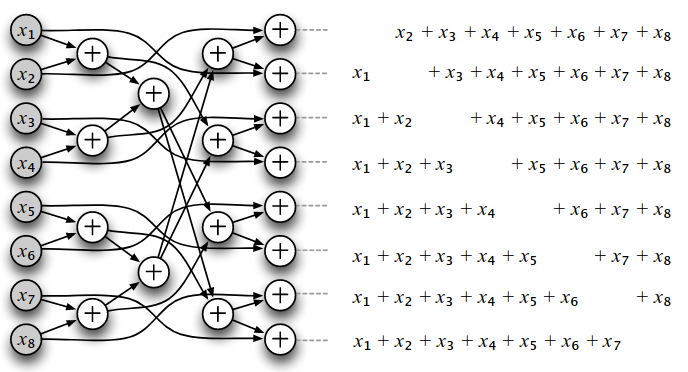
\includegraphics[width=7.5cm]{aplicacion}
        \caption{Un ejemplar de Ensemble Computing (derecha) y un circuito que lo resuelve (izquierda).}
    \end{figure}
\end{frame}

%------------------------------------------------

\begin{frame}
\frametitle{Referencias}
\footnotesize{
\begin{thebibliography}{99} % Beamer does not support BibTeX so references must be inserted manually as below
\bibitem[]{p1} Garey \& Johnson, \\
\emph{Computers and Intractactability, A Guide to the Theory of NP-Completeness}.
\newblock (1979). Estados Unidos de América: Freeman.
\newblock \url{https://sites.google.com/a/ciencias.unam.mx/cco-2019-1/recursos/\%5BGarey-Johnson\%5D\%20Computers\%20and\%20Intractability.djvu?attredirects=0\&d=1}

\end{thebibliography}
}
\end{frame}

%------------------------------------------------

\begin{frame}
\huge{\centerline{Gracias por su atención.}}
    \begin{figure}[H]
        \centering
        
\includegraphics[width=8cm]{computer_science}
    \end{figure}
\end{frame}

%----------------------------------------------------------------------------------------

\end{document}